\documentclass[a4paper, 11pt]{beamer}

\usepackage{polski}
\usepackage[utf8]{inputenc}
\usepackage{units}

\mode<presentation> {
	\usetheme{Frankfurt}
	\setbeamercovered{transparent}
	\usecolortheme{default}
}

\title{Ekonometria Dynamiczna}
\subtitle{Model liniowy jako narzędzie analizy szeregów czasowych}
\author{mgr Paweł Jamer\thanks{pawel.jamer@gmail.com}}

\begin{document}

	\begin{frame}
		\titlepage
	\end{frame}
	
	\section{Model}

	\begin{frame}{Model regresji wielorakiej}
		\textbf{Równanie modelu:}
		\[
			Y_t = \beta_0 + \sum_{i=1}^{k} \beta_i X_{i,t} + \epsilon_{t},
		\]
		dla $t = 1, 2, \ldots, T.$
		\newline\newline
		\textbf{Założenia:}
		\begin{itemize}
			\item $\epsilon_t \sim \mathcal{N}\left(0, \sigma^2\right), t = 1, 2, \ldots, T;$
			\item $\epsilon_t$ oraz $\epsilon_s$ są niezależne dla dowolnych $s$ i $t$ takich, że $s \neq t;$
			\item $\epsilon_t$ oraz $x_s$ są niezależne dla dowolnych $s$ i $t;$
			\item $x_t$ oraz $x_s$ są nieskorelowane dla dowolnych $s$ i $t$ takich, że $s \neq t.$
		\end{itemize}
	\end{frame}
	
	\begin{frame}{Model regresji wielorakiej (macierzowo)}
		\textbf{Równanie modelu:}
		\[
			\boldsymbol{Y} = \boldsymbol{X} \boldsymbol{\beta} + \boldsymbol{\epsilon},
		\]
		gdzie
		\begin{itemize}
			\item $\boldsymbol{Y} = \left[\begin{matrix}
				Y_1 & Y_2 & \cdots & Y_T
			\end{matrix}\right]^{\prime}$ --- wektor odpowiedzi;
			\item $\boldsymbol{\beta} = \left[\begin{matrix}
				\beta_0 & \beta_1 & \ldots & \beta_k
			\end{matrix}\right]^{\prime}$ --- wektor parametrów;
			\item $\boldsymbol{\epsilon} = \left[\begin{matrix}
				\epsilon_1, \epsilon_2, \ldots, \epsilon_T
			\end{matrix}\right]^{\prime}$ --- wektor błędów;
			\item $\boldsymbol{X} = \left[\begin{matrix}
				1 & X_{1,1} & X_{2,1} & \cdots & X_{k,1}\\
				1 & X_{1,2} & X_{2,2} & \cdots & X_{k,2}\\
				\vdots & \vdots & \vdots & \ddots & \vdots\\
				1 & X_{1,T} & X_{2,T} & \cdots & X_{k,T}
			\end{matrix}\right]$ --- macierz eksperymentu.
		\end{itemize}
	\end{frame}

	\section{Estymacja}

	\begin{frame}{Metoda Najmniejszych Kwadratów (MNK)}
		\begin{alert}{\textbf{Idea MNK}}
			Chcemy tak dobrać parametry $\beta_0, \beta_1, \ldots, \beta_k$ modelu regresji wielorakiej,
			aby minimalizować sumaryczną odległość punktów $Y_1, Y_2, \ldots, Y_T$ od krzywej regresji.
		\end{alert}
		\begin{block}{\textbf{Funkcja celu MNK}}
			\[
				Q\left(\boldsymbol{\beta}\right) = 
				\left(\boldsymbol{Y} - \boldsymbol{X} \boldsymbol{\beta}\right)^{\prime}
				\left(\boldsymbol{Y} - \boldsymbol{X} \boldsymbol{\beta}\right)
				\rightarrow \min.
			\]
		\end{block}
		\begin{block}{\textbf{Estymator MNK}}
			\[
				\hat{\boldsymbol{\beta}} = \left(\boldsymbol{X}^{\prime} \boldsymbol{X}\right)^{-1} \boldsymbol{X}^{\prime} \boldsymbol{Y}.
			\]
		\end{block}
	\end{frame}
	
	\begin{frame}{Właściwości MNK}
		Estymator MNK jest \textbf{nieobciążony}, tzn. \[
			\mathbb{E}\left(\hat{\boldsymbol{\beta}}\right) = \boldsymbol{\beta}.
		\]
		Macierz kowariancji estymatora MNK przyjmuje postać \[
			\mbox{Cov}\left(\hat{\boldsymbol{\beta}}\right) = \sigma^2 \left(\boldsymbol{X}^{\prime} \boldsymbol{X}\right)^{-1}.
		\]
		\begin{block}{\textbf{Twierdzenie Gaussa-Markowa}}
			W modelu regresji wielorakiej estymator MNK jest estymatorem o minimalnej wariancji w klasie estymatorów liniowych nieobciążonych.
		\end{block}
		\begin{block}{\textbf{Twierdzenie}}
			W modelu regresji wielorakiej estymator MNK jest równy estymatorowi największej wiarogodności.
		\end{block}
	\end{frame}
	
	\section{Diagnostyka}
	
	\begin{frame}{Residua}
		\begin{block}{\textbf{Wartości dopasowane}} \[
				\hat{\boldsymbol{Y}} = \boldsymbol{X} \hat{\boldsymbol{\beta}}.
			\]
		\end{block}
		Na potrzeby teorii: \[
			\hat{\boldsymbol{Y}} = \boldsymbol{H} \boldsymbol{Y},
		\]
		gdzie
		\begin{itemize}
		  \item $\boldsymbol{H} = \boldsymbol{X} \left(\boldsymbol{X}^{\prime} \boldsymbol{X}\right)^{-1} \boldsymbol{X}^{\prime}$ --- macierz daszkowa.
		\end{itemize}
		\begin{block}{\textbf{Residua}}
			\[
				\boldsymbol{e} = \boldsymbol{Y} - \hat{\boldsymbol{Y}}
			\]
		\end{block}
		\begin{itemize}
			\item $\mathbb{E}\left(\boldsymbol{e}\right) = \boldsymbol{0},$
			\item $\mbox{Cov}\left(\boldsymbol{e}\right) = \sigma^2 \left(\boldsymbol{I} - \boldsymbol{H}\right).$
		\end{itemize}
		\begin{alert}{\textbf{Intuicja}}
			Residua $\boldsymbol{e}$ to próbkowy odpowiednik błędów modelu $\boldsymbol{\epsilon}.$
		\end{alert}
	\end{frame}
	
	\begin{frame}{Normalność rozkładu (graficznie)}
		\begin{itemize}
			\item Residua w funkcji wartości dopasowanych. Oczekujemy
			\begin{itemize}
				\item średniej równej zero,
				\item jednorodnej wariancji.
			\end{itemize}
			\item Wykres kwantylowy standaryzowanych residuów. Oczekujemy
			\begin{itemize}
				\item ułożenia się obserwacji na linii $y=x.$
			\end{itemize}
		\end{itemize}
		\begin{figure}
			\centering
			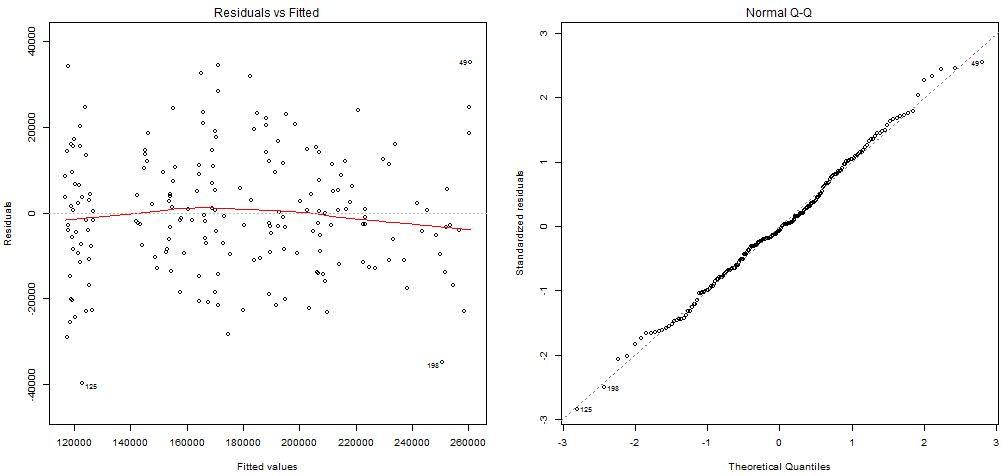
\includegraphics[scale=0.45]{gfx/normality}
		\end{figure}
	\end{frame}
	
	\begin{frame}{Normalność rozkładu (test)}
		Niech $e_1, e_2, \ldots, e_T \sim F.$
		
		\begin{block}{\textbf{Pytanie}}
			Czy dystrybuanta $F$ jest dystrybuantą rozkładu normalnego $F_{\mathcal{N}}?$
		\end{block}

		Testujemy hipotezę: \[
			\begin{cases}
				H_{0}: & F = F_{\mathcal{N}}\\
				H_{1}: & F \neq F_{\mathcal{N}}
			\end{cases}
		\]
		
		\begin{block}{\textbf{Test Shapiro-Wilka}} \[
				W = \frac{
					\left[
						\sum_{t=1}^{\left[\nicefrac{T}{2}\right]}a_{T-t+1}\left(e_{T-t+1:T}-e_{t:T}\right)
					\right]^{2}
				}{
					\sum_{t=1}^{T} e_{t}^{2}
				}
			\]
		\end{block}
		
		\begin{alert}{Zaleta}
			Test Shapiro-Wilka jest mało wrażliwy na typowe problemy regresji.
		\end{alert}
		
	\end{frame}
	
	\begin{frame}{Współczynnik determinacji}
		\textbf{Definiujemy}:
		\begin{itemize}
			\item $\mbox{SST} = \sum_{t=1}^{T} \left(Y_t - \overline{Y}\right)^2,$
			\item $\mbox{SSR} = \sum_{t=1}^{T} \left(\hat{Y}_t - \overline{Y}\right)^2,$
			\item $\mbox{SSE} = \sum_{t=1}^{T} \left(Y_t - \hat{Y}_t\right)^2.$
		\end{itemize}
		\textbf{Zachodzi}: \[
			\mbox{SST} = \mbox{SSR} + \mbox{SSE}.
		\]
		\begin{alert}{\textbf{Obserwacja}}
			Jeśli wykres rozproszenia silnie skupia się wokół prostej regresji, to \[
				\mbox{SSE} \ll \mbox{SST}.
			\]
		\end{alert}
		\begin{block}{\textbf{Współczynnik determinacji}}
			\[
				R^2 = 1 - \frac{\mbox{SSE}}{\mbox{SST}}
			\]
		\end{block}
	\end{frame}
	
	\begin{frame}{Istotność równania regresji}
		\begin{block}{\textbf{Pytanie}}
			Czy równanie regresji ma sens jako całość?
		\end{block}
		
		Testujemy hipotezę: \[
			\begin{cases}
				H_{0}: & \hat{\beta}_1 = \hat{\beta}_2 = \ldots = \hat{\beta}_k = 0\\
				H_{1}: & \left(\exists i\right) \hat{\beta}_i \neq 0
			\end{cases}
		\]
		
		\begin{block}{\textbf{Test F}}
			\[
				F=\frac{\nicefrac{SSR}{k}}{\nicefrac{SSE}{\left(T-k-1\right)}} \sim \mathbb{F}^{\left[k, T-k-1\right]}
			\]
		\end{block}
	\end{frame}
	
	\begin{frame}{Istotność parametrów}
		\begin{block}{\textbf{Pytanie}}
			Czy zmienna $X_i$ ma istotny wpływ na zmienną $Y?$
		\end{block}
		
		Testujemy hipotezę: \[
			\begin{cases}
				H_{0}: & \hat{\beta}_i = 0\\
				H_{1}: & \hat{\beta}_i \neq 0
			\end{cases}
		\]
		
		\begin{block}{\textbf{Test t}} \[
			t_i = \frac{\hat{\beta}_i}{\mbox{SE}_{\hat{\beta}_{i}}} \sim t^{\left[T-k-1\right]}
		\]
		\end{block}
	\end{frame}
	
	\begin{frame}{Współliniowość}
		
		\begin{alert}{\textbf{Problem}}
			Jeśli wśród zmiennych objaśniających występują zmienne współliniowe,
			to macierz $\boldsymbol{X}^{\prime}\boldsymbol{X}$ nie jest odwracalna.
		\end{alert}
		
		\begin{block}{\textbf{Czynnik inflacji wariancji}}
			\[
				\mbox{VIF}_i = \frac{1}{1 - R^2_i},
			\]
			gdzie
			\begin{itemize}
				\item $R^2_i$ --- współczynnik determinacji w modelu,
					w którym zmienną objaśnianą jest $X_i,$ a zmiennymi objaśniającymi
					zmienne $X_1, \ldots, X_{i-1}, X_{i+1}, \ldots, X_k.$
			\end{itemize}
		\end{block}
		\begin{alert}{\textbf{Heurystyka}}
			Kiedy $\mbox{VIF}_j > 10,$ to zmienna $j$ wykazuje dużą współliniowość ze zmiennymi pozostałymi.
		\end{alert}
		
	\end{frame}

	\section{Selekcja}
	
	\begin{frame}{Skorygowany współczynnik determinacji}

		\begin{alert}{\textbf{Problem}}
			Współczynnik $R^2$ rośnie wraz z dokładaniem kolejnych zmiennych do modelu.
		\end{alert}

		\begin{block}{\textbf{Skorygowany współczynnik determinacji}}
			\[
				\overline{R}^2 = 1 - \frac{\nicefrac{\mbox{SSE}}{\left(T - k - 1\right)}}{\nicefrac{\mbox{SST}}{\left(T - 1\right)}}
			\]
		\end{block}
	\end{frame}

	\begin{frame}{Kryteria informacyjne}
		\begin{alert}{\textbf{Problem}}
			Wzrost liczby obserwacji $T$ wywiera zbyt silny wpływ na skorygowany wpsółczynnik determinacji $\overline{R}^2.$
		\end{alert}
	
		\begin{block}{\textbf{Kryterium informacyjne Akaike (AIC)}}
			\[
				\mbox{AIC} = T \ln \frac{\boldsymbol{e}^{\prime}\boldsymbol{e}}{T} + 2\left(k + 1\right)
			\]
		\end{block}
		
		\begin{block}{\textbf{Bayesowskie kryterium informacyjne (BIC)}}
			\[
				\mbox{BIC} = T \ln \frac{\boldsymbol{e}^{\prime}\boldsymbol{e}}{T} + \left(k + 1\right) \ln T
			\]
		\end{block}
		
	\end{frame}
	
	\begin{frame}{Selekcja modelu}
		\begin{block}{\textbf{Pytanie}}
			Jak ze zbioru zmiennych objaśniających $X_1, X_2, \ldots, X_k$ wybrać w sposób automatyczny te,
			które w najlepszy sposób opisują zmienną odpowiedzi $Y?$
		\end{block}
		
		\begin{itemize}
			\item \textbf{forward}: zaczynamy od modelu pustego i w kolejnych krokach wybieramy spośród zmiennych jeszcze nie wybranych tą, która ma
				najbardziej pozytywny wpływ na kryterium.
			\item \textbf{backward}: zaczynamy od modelu pełnego i w kolejnych krokach odrzucamy spośród zmiennych znajdujących się w modelu tą, której
				brak wywrze najbardziej istotny wpływ na kryterium informacyjne.
			\item \textbf{both}: naprzemienne stosowanie metod poprzednich.
		\end{itemize}
	\end{frame}
	
	\section{Predykcja}

	\begin{frame}{Predykcja}
		\textbf{Niech}:
		\begin{itemize}
			\item $\hat{\boldsymbol{\beta}}$ --- wektor estymatorów MNK regresji wielorakiej.
			\item $\boldsymbol{X}_{new}$ --- macierz zawierająca nowe wartości zmiennych objaśniających,
				dla których nie są znane wartości zmiennej objaśnianej.
		\end{itemize}
		
		\begin{alert}{Problem}
			Chcemy wyznaczyć prawdopodobne wartości zmiennych objaśnianych $\hat{Y}_{new}$
		\end{alert}
		
		
		\begin{block}{\textbf{Predykcja}}
			\[
				\hat{Y}_{new} = \boldsymbol{X}_{new} \hat{\boldsymbol{\beta}}
			\]
		\end{block}
		
		\textbf{Przedział ufności dla predykcji}:
		
		\[
			\hat{Y}_{new} - t^{\left[T - k - 1\right]}_{\nicefrac{\alpha}{2}} \hat{\mbox{SE}}_{new} \leq Y_{new} \leq \hat{Y}_{new} + t^{\left[T - k - 1\right]}_{\nicefrac{\alpha}{2}} \hat{\mbox{SE}}_{new}
		\]
	\end{frame}

	\section*{}

	\begin{frame}
		\center
		\Huge \bfseries
		Pytania?
	\end{frame}

	\begin{frame}
		\center
		\Huge \bfseries
		Dziękuję za uwagę!
	\end{frame}

\end{document}